\documentclass{beamer}
\usetheme{Madrid}
\usecolortheme{whale}

\usepackage{appendixnumberbeamer}
\usepackage{multimedia}
\usepackage{braket}
\usepackage{array}
\definecolor{mypurple}{RGB}{255,0,255}

\newcommand{\abs}[1]{\left\lvert #1 \right\rvert}
\graphicspath{ {Graphics/}  }
\setbeamerfont{caption}{size=\scriptsize}

\title[Sympathetic Cooling Ba/Yb]{Sympathetic Cooling and Reordering in Multiple Trapped Ion Species Chains}
\subtitle{Exploring Using Barium Ions to Sympathetically Cool a Ytterbium Ion Quantum Computer}
\author[J. Wright]{John Wright}
\institute[UW] {
	Department of Physics \\
	University of Washington
}
\date[June 2014]{June 5, 2014}

\begin{document}

\begin{frame}[plain]
\titlepage
\end{frame}

\section{MUSIQC}
\begin{frame}{MUSIQC - Introduction}
Modular Universal Scalable Ion-Trap Quantum Computer
\begin{itemize}
	\item Final deliverable planned to have up to 80 qubits
	\item Plan to have largest possible ion chains in each trap	and scale further by linking ions via radiated photons
\end{itemize}
\centerline{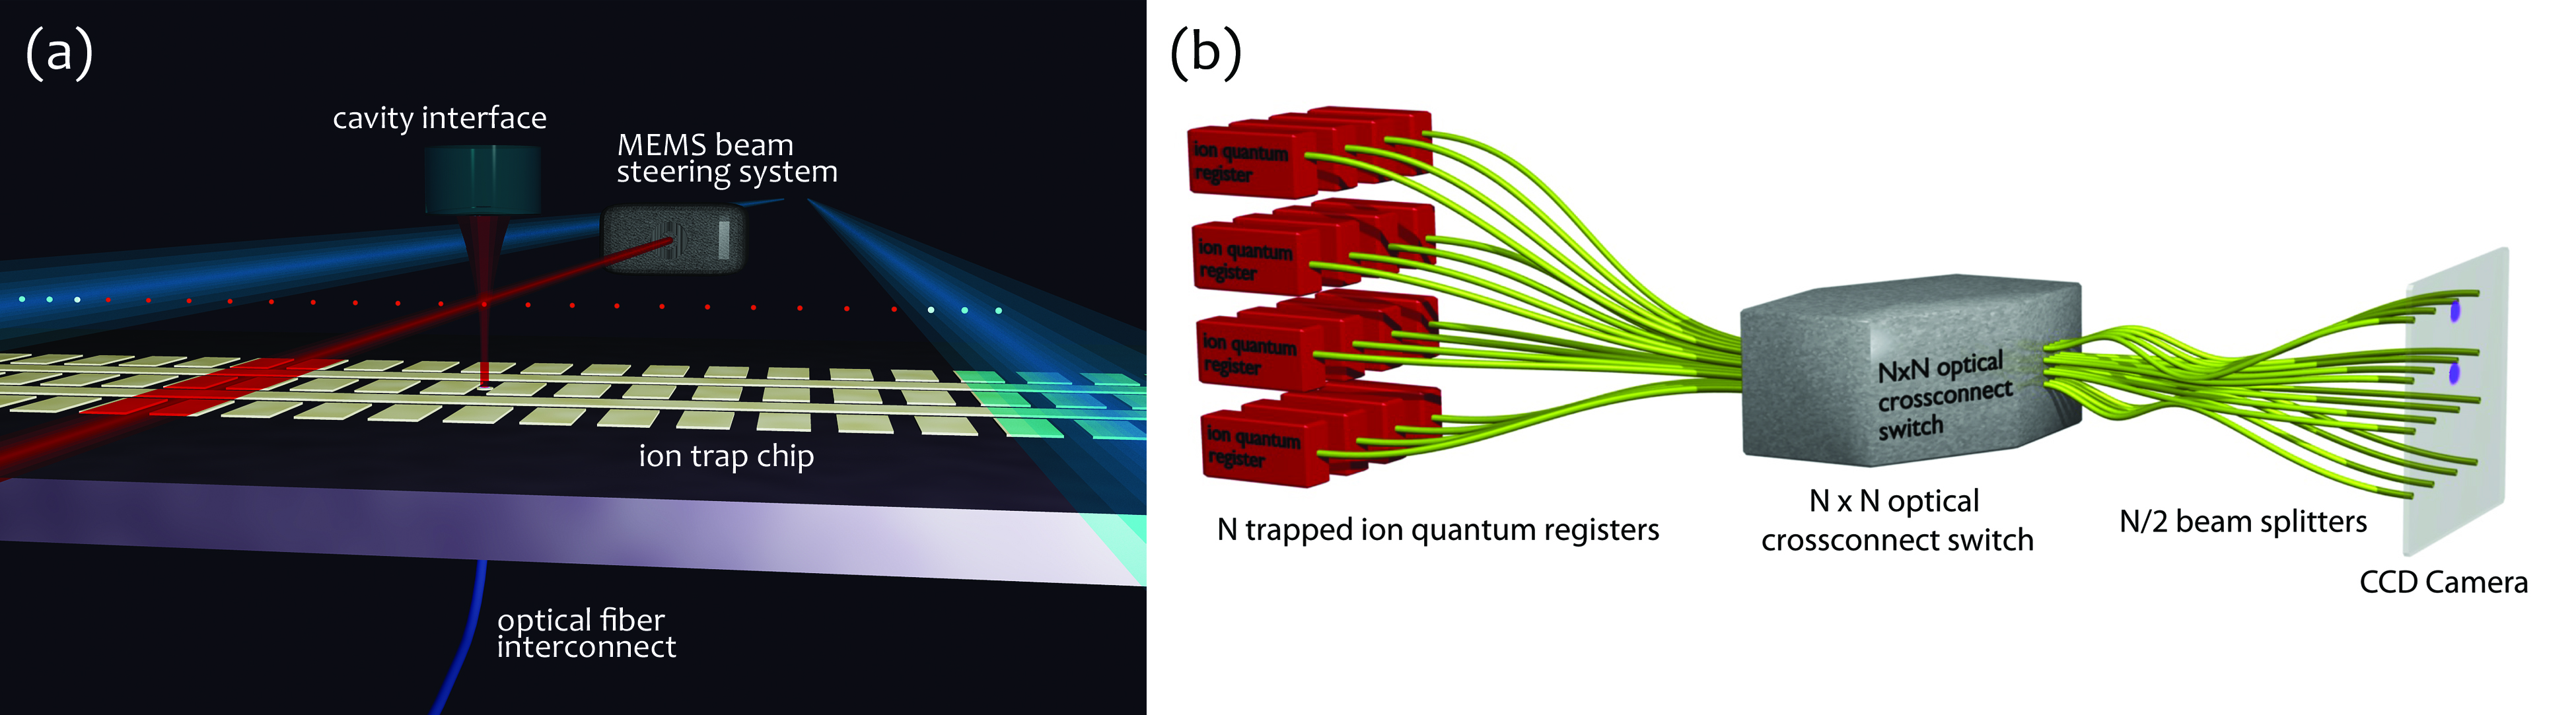
\includegraphics[height=0.38\textheight]{MUSIQC-plan}}
\let\thefootnote\relax\footnote[frame]{C.Monroe, et al, 2012, arXiv:1208.0391}
\end{frame}

\begin{frame}{MUSIQC - Using Multiple Ion Species}
\begin{columns}
	\begin{column}{0.4\textwidth}
		\centerline{\includegraphics[width=0.9\textwidth]%
			{energylevels-BaYb}}
	\end{column}
	\begin{column}{0.6\textwidth}
		\begin{itemize}
			\item Light from Barium's cooling transition (493nm) is easily transferred long distances via optical fiber
			\item Yb-171 has long lived hyperfine states that can easily be frequency initialized and used for motional gates
			\item Separating these tasks to different species reduces the possibility for crosstalk
			\item Information is transferred between ions using ion crystal motional modes
		\end{itemize}
	\end{column}
\end{columns}
\end{frame}

\section[BaYb]{Barium-Ytterbium System}
\begin{frame}{Trapping Barium and Ytterbium}
\centerline{\includegraphics[width=0.9\textwidth]%
	{example_data_7_3}}
\begin{itemize}
	\item Crystal contains 4 cooled, bright Ba ions and 3 dark Yb ions
	\item We have a new observable compared to most trapped ion experiments - ion species configuration
	\item Knowing when the ions spontaneously reorder tells us something about the average energy in their motional degrees of freedom
	\item Measuring this directly is possible one mode at a time, but we want to scale to dozens of ions
\end{itemize}
\end{frame}

\begin{frame}{Sympathetic Cooling with Barium}
\begin{columns}
	\begin{column}{0.4\textwidth}
		\centerline{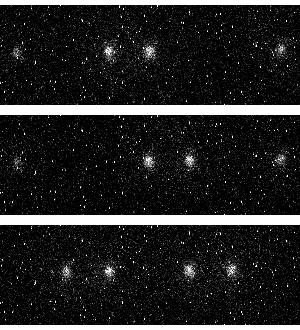
\includegraphics[width=0.9\textwidth]{example_data}}
	\end{column}
	\begin{column}{0.6\textwidth}
		\begin{itemize}
			\item We begin with a Doppler cold chain of mixed Barium and Ytterbium ions
			\item The cooling lasers are mechanically shuttered for varying periods of time
			\item Software integrated with our EMCCD automatically detects whether the chain has reordered after the cooling lasers are unblocked
		\end{itemize}
	\end{column}
\end{columns}
\end{frame}

\section[Reorder]{Ion Reordering Experiment}
\begin{frame}{Ion Reordering Measurements}
\centerline{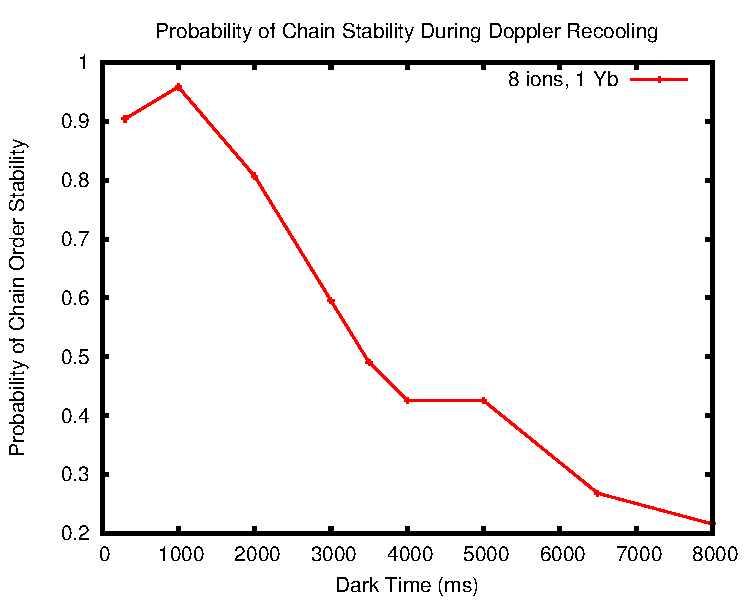
\includegraphics[width=0.8\textwidth]{data}}
\end{frame}

\begin{frame}{Ion Reordering Simulations}
\centerline{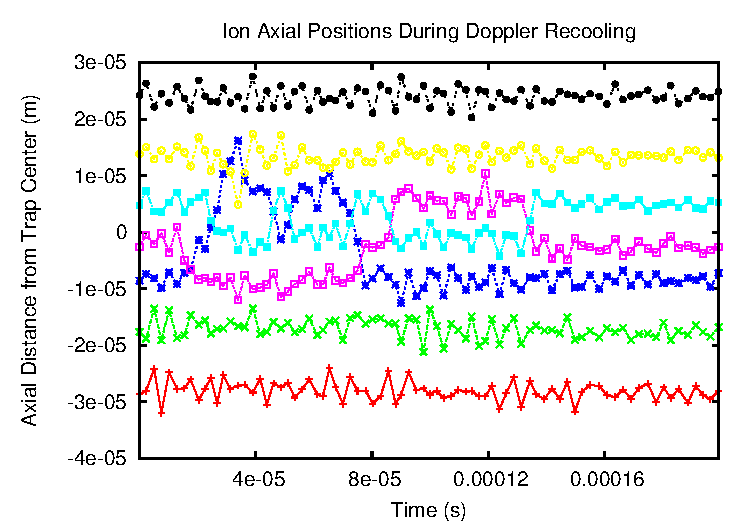
\includegraphics[width=0.6\textwidth]{simulation}}
\begin{itemize}
	\item Simulate classical ion motion starting at a given average kinetic energy and laser cooling to crystallization
	\item Comparing probability of detectable reordering between simulation and experiment gives conversion between dark time and energy
\end{itemize}
\end{frame}

\begin{frame}{Results}
\centerline{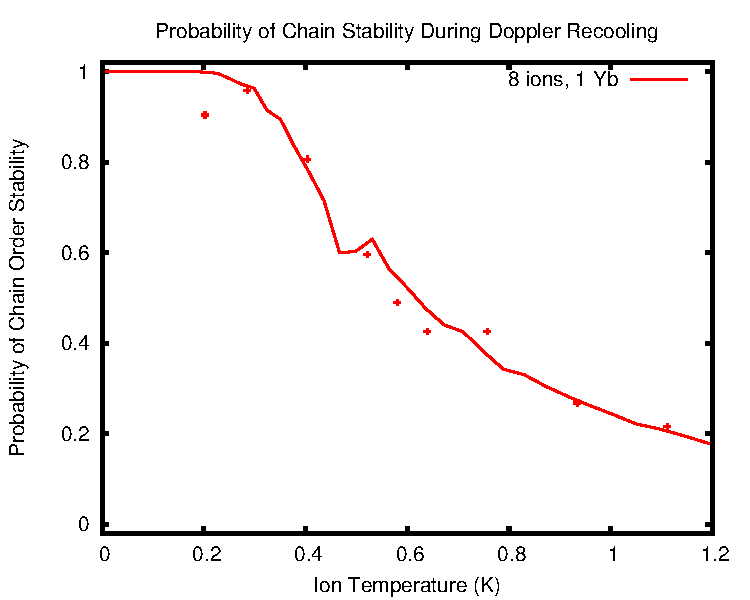
\includegraphics[width=0.6\textwidth]{results}}

\begin{block}{Fit Parameters}
	\centerline{\begin{tabular*}{0.8\textwidth}{@{\extracolsep{\fill}}lll}
	Initial Temperature & Heating Rate \\ \hline 
	\rule{0pt}{3ex} \(0.167 K\) & \(0.118 \frac{K}{s}\) \\
	\end{tabular*}}
\end{block}
\end{frame}

\begin{frame}{Future Directions}
\begin{itemize}
	\item Can we use this sharp slope in reordering to fine tune parameters to minimize the heating rate?
	\item How stable is a single ground state cooled motional degree of freedom in our quantum computing ions?
	\item How long can we perform quantum operations using that motional state while EIT cooling one species?
\end{itemize}
\end{frame}

\begin{frame}{Future Directions}
How stable are different configurations of ions? Are the stable configurations optimal for keeping the dark ions cool?
\centerline{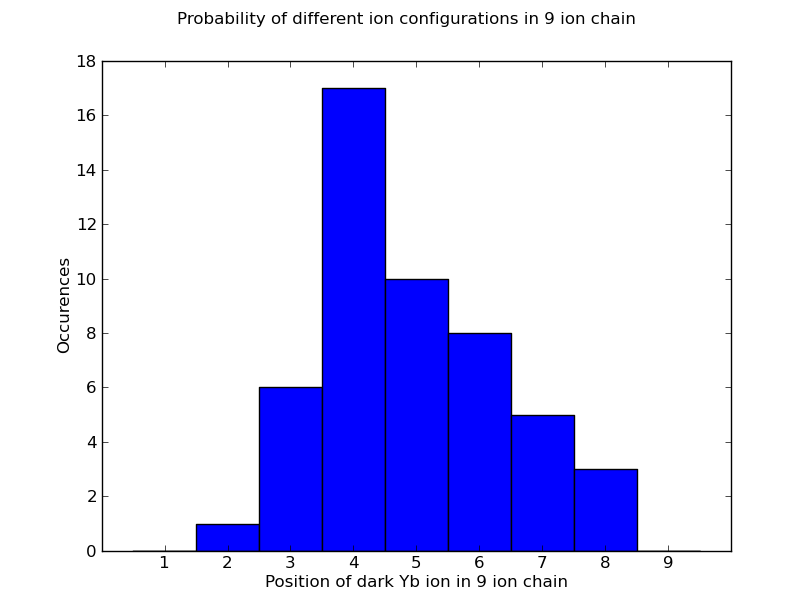
\includegraphics[width=0.8\textwidth]{orderings_9_1}}
\end{frame}

\section[]{Conclusions}
\begin{frame}{Conclusions}
\begin{itemize}
	\item MUSQIC program plans to implement a quantum computer with up to 80 qubits which would be capable of outperforming classical computers on specific tasks
	\item Using mixed species chains allows longer quantum operations to be carried out by continuously cooling one ion species
	\item Certain configurations of cooling ions may help preserve the motional states of quantum computing ions longer
\end{itemize}
\end{frame}

\begin{frame}{Thank You}
PI: Boris Blinov
\begin{block}{MUSQIC}
\begin{tabular*}{0.9\textwidth}{ccc}
Tomasz Sakrejda & Richard Graham & Zichao Zhou \\
\end{tabular*}
\end{block}

\begin{block}{Ion Trappers}
\begin{tabular*}{0.9\textwidth}{ccc}
Tom Noel & Carolyn Auchter & Chen-Kuan Chou \\
Matt Hoffman & Spencer Williams & Anupriya Jayakumar \\
Matt Bohman
\end{tabular*}
\end{block}

\begin{columns}
\begin{column}{0.5\textwidth}
	
\includegraphics[width=0.9\textwidth]{musiqc_logo}
\end{column}
\begin{column}{0.5\textwidth}
	
\includegraphics[width=0.9\textwidth]{iarpa}
\end{column}
\end{columns}
\end{frame}

\end{document}
